% CS F407 Artificial Intelligence: final project report (limit: 4 pages, everything except references).
\documentclass[11pt,a4paper,twocolumn]{article}

\usepackage[margin=2cm,columnsep=0.8cm]{geometry}
\usepackage[T1]{fontenc}
\usepackage{lmodern}
\usepackage{microtype}
\usepackage{amsmath,amssymb}
\usepackage{graphicx}
\usepackage{booktabs}
\usepackage{tabularx}
\usepackage{enumitem}
\usepackage{titlesec}
\usepackage[hidelinks]{hyperref}

\titleformat{\section}{\normalsize\bfseries}{\thesection}{0.6em}{}
\titlespacing*{\section}{0pt}{1.2ex plus 0.3ex}{0.6ex}
\setlist{nosep,leftmargin=*}
\setlength{\parskip}{0.3ex}
\raggedbottom

\newcommand{\coursename}{CS F407 Artificial Intelligence, AY 2026--27 Semester I}
\newcommand{\teamno}{Team MARS}
\newcommand{\githuburl}{https://github.com/malharbhalerao/folk-restore}

\begin{document}

\twocolumn[{%
\begin{center}
  {\large\bfseries folk-restore: Multi-Stage Digital Restoration of Indian Folk Paintings with Calibrated Confidence Maps}\\[1ex]
  \teamno\\
  Malhar Bhalerao (2024A8PS1439G), Shriya Kulkarni (2024A7PS0486G), Aditya Vilas (2024A7PS0002G)\\[0.5ex]
  {\small \coursename, BITS Pilani, K.K. Birla Goa Campus}\\[1.5ex]
  \begin{minipage}{0.85\textwidth}
    \small
    \centerline{\bfseries Abstract}\vspace{0.5ex}
    Museum folk paintings suffer cracks, paint loss, stains and fading, and no labelled damage data exist for them. We build a
    four-stage pipeline (damage segmentation, inpainting, colour de-fading, super-resolution) trained only on a procedural damage
    simulator, and add a per-pixel confidence map that tells a conservator which fills are speculative. A segmenter trained with
    unlabelled design lines as hard negatives and wall-plaster damage raises union Dice on wall-style damage from 0.32 to 0.78;
    fine-tuning Big-LaMa gains 0.7~dB over zero-shot; an inpainter-disagreement signal fitted on validation tiles predicts true
    repair error with Spearman $\rho=0.71$ (tile level 0.94). Several expected gains did not appear (CLAHE features, a GAN
    de-fader, a discriminator-based signal), and we report them. Real-painting results are qualitative.
  \end{minipage}
\end{center}
\vspace{1.5ex}
}]

\section{Introduction}
Digital restoration gives conservators a non-destructive preview of a painting's earlier state. Our input is a photograph of a damaged
painting (Madhubani, Pattachitra, Warli, Kalamkari, or Mandawa wall paintings); the output is a restored high-resolution PNG plus a matrix
of per-pixel confidence ($1$ = original paint or well-supported fill, $0$ = speculative). The difficulty is that there is no paired
damaged/clean data, and a false detection makes the inpainter \emph{erase real design}. Contributions: (i) a damage simulator with
unlabelled decoy design lines, plaster-wall damage and photographic degradations; (ii) a measured comparison of Telea, zero-shot and
fine-tuned LaMa and diffusion inpainting; (iii) a confidence map whose fusion weights are fitted against true error; (iv) honest negative
results on CLAHE, Pix2Pix and discriminator-based uncertainty.

\section{Background and related work}
We combine classical image processing (CLAHE~\cite{zuiderveld1994clahe}, black-hat morphology, Telea inpainting~\cite{telea2004}) with
a U-Net~\cite{ronneberger2015unet}, the large-mask inpainter LaMa built on Fourier convolutions~\cite{suvorov2022lama}, latent-diffusion
inpainting~\cite{rombach2022ldm}, conditional GANs for image translation (Pix2Pix~\cite{isola2017pix2pix}) and Real-ESRGAN super-resolution~\cite{wang2021realesrgan}. Global colour transfer~\cite{reinhard2001} is our de-fading baseline.
Uncertainty is usually studied for classification; for generative repair we use ensemble-style disagreement and calibrate it on data where the truth is known.

\section{Method}
\textbf{M1 Segmentation.} A U-Net (ResNet-34, ImageNet weights) takes five channels (RGB, CLAHE of $L$, black-hat of $L$) and predicts three sigmoid maps
(crack, loss, stain); loss is BCE+Dice. Training damage is synthesised on the fly (\texttt{degrade.py}): branching random-walk cracks, thresholded-noise
flaking, tide-line stains, LAB fading, and, new in v3, \emph{(a)} unlabelled decoy strokes (vines, outlines, dotted borders) on 40\% of tiles so smooth uniform
strokes are learnt as design and jagged branching ones as cracks, \emph{(b)} plaster flaking with ochre/brick underlayer, salt blooms and rain streaks,
\emph{(c)} damage rendered at 0.5--2$\times$ scale, \emph{(d)} phone-photo blur/noise/JPEG/uneven light. Masks are the union of classes, closed, filtered and dilated.

\textbf{M2 Inpainting.} Big-LaMa (51\,M parameters, TorchScript) is fine-tuned for 8 epochs with masked L1 (weight 10) + VGG perceptual + spectral-norm PatchGAN hinge loss
(ramped to 0.05) on simulated-damage tiles plus random large blobs; lr $2\!\times\!10^{-5}$. We also run Stable Diffusion~1.5 inpainting (fp16, 25 steps) and always composite the original outside the mask.

\textbf{M3 Colour.} A U-Net predicts a LAB residual added to the input (zero-initialised head $\Rightarrow$ identity at start), L1 loss, 15\% unfaded samples.
Variants: Pix2Pix (LSGAN PatchGAN, $\lambda_{L1}=100$) and a \emph{margin-reference} input (LAB mean/std of an unfaded strip, as hidden under a frame).

\textbf{M4 Super-resolution and confidence.} Real-ESRGAN x4 (own RRDBNet loader, official weights) in overlapping tiles with linear blending. The confidence map fuses four signals
inside repaired holes: segmenter entropy, depth inside the hole, \emph{disagreement} between three LaMa runs (original, mirrored, rotated; CIELAB spread), and PatchGAN realness
of the fill. Outside holes only entropy applies. Weights are fitted by non-negative least squares from signals to $|{\rm restored}-{\rm clean}|$ on validation tiles
and scored on test tiles.

\section{Experimental setup}
\textbf{Data.} 124 open-licence images after de-duplication (Kalamkari 31, Madhubani 20, Pattachitra 41, Warli 32; Wikimedia Commons, Cleveland Museum, CC0/PD), split \emph{by image}
93/12/19 into 5{,}872/763/1{,}192 tiles of $512^2$. Fixed seeded synthetic val/test sets (200 tiles each) exist in paper style and wall style. The dataset provided by Prof.\ Tirtharaj Dash (67 Mandawa wall-painting photographs,
damaged only, no ground truth) was never trained or tuned on; a dHash check found 0 overlaps with our 135 training/demo images.

\noindent\textbf{Metrics.} Dice (mean per tile, bootstrap 95\% CI), PSNR on the repaired region, LPIPS and SSIM on the tile, CIEDE2000 $\Delta E_{00}$, Spearman $\rho$ and AUROC for confidence vs.\ error.

\noindent\textbf{Hardware/software.} One RTX 3050 (6\,GB), PyTorch 2.6, segmentation-models-pytorch, diffusers; all runs seeded. Code and commands: repository README.

\section{Results}
\begin{figure*}[!t]
\centering
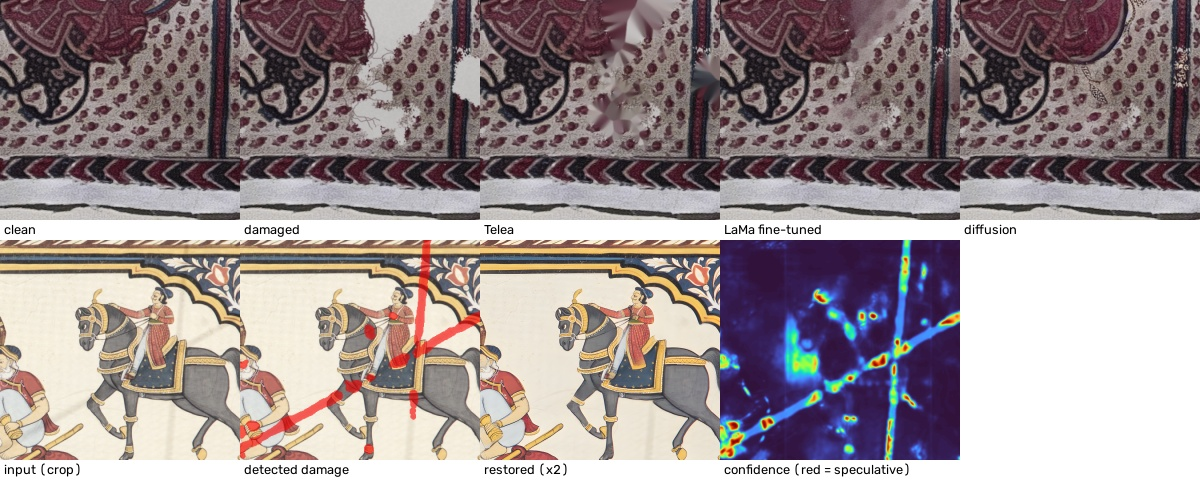
\includegraphics[width=0.78\textwidth]{qualitative.jpg}
\caption{Top: simulated tile (clean, damaged, Telea, fine-tuned LaMa, diffusion). Bottom: Mandawa wall photograph, crop around detected damage (input, detected damage, restored $\times2$, confidence; red = speculative).}
\label{fig:qual}
\end{figure*}

\textbf{Segmentation (Table~\ref{tab:seg}).} The midsem model (v1) collapses on wall-style damage; v3 fixes this at a small cost on paper-style tiles. In the ablation, plain RGB input matched or beat CLAHE+black-hat (clearly so for v1), so the proposal's CLAHE step gave no measurable benefit on simulated damage.

\begin{table}[h]
\centering
\small
\resizebox{\columnwidth}{!}{\begin{tabular}{lcc}
\toprule
Union Dice (95\% CI) & paper test & wall test \\
\midrule
v1 CLAHE+black-hat & 0.83 (.81--.85) & 0.32 (.30--.36) \\
v3 CLAHE+black-hat & 0.80 (.78--.82) & 0.78 (.75--.80) \\
v1 RGB only (ablation) & 0.87 (.85--.88) & -- \\
v3 RGB only (ablation) & 0.79 (.76--.81) & 0.79 (.76--.82) \\
\bottomrule
\end{tabular}}
\caption{Segmentation on 200 simulated tiles per set (higher is better).}
\label{tab:seg}
\end{table}

\textbf{Inpainting (Table~\ref{tab:inp}).} Fine-tuning improves repaired-region PSNR by $+0.8$/$+0.7$\,dB (oracle/predicted masks) but LPIPS is not better. Diffusion is clearly worse on every metric (it invents plausible but different content), so we keep it only as a comparison and as a candidate uncertainty source.

\begin{table}[h]
\centering
\small
\resizebox{\columnwidth}{!}{\begin{tabular}{lccc}
\toprule
Method (predicted masks) & PSNR$\uparrow$ & LPIPS$\downarrow$ & SSIM$\uparrow$ \\
\midrule
No restoration & 16.01 & 0.107 & 0.939 \\
Telea & 19.87 & 0.074 & 0.944 \\
LaMa zero-shot & 21.64 & 0.046 & 0.949 \\
LaMa fine-tuned & 22.36 & 0.046 & 0.955 \\
Diffusion (SD 1.5)$^\dagger$ & 19.38 & 0.062 & 0.933 \\
\bottomrule
\end{tabular}}
\caption{Inpainting on 100 test tiles (PSNR in the repaired region; LPIPS/SSIM on the tile). Oracle masks: Telea 19.70, zero-shot 22.97, fine-tuned 23.74\,dB. $^\dagger$First 50 tiles only (slow); on those tiles fine-tuned LaMa scores 22.56\,dB / 0.050 and Telea 20.02\,dB / 0.079.}
\label{tab:inp}
\end{table}

\textbf{Colour (Table~\ref{tab:col}).} The de-fader cuts $\Delta E_{00}$ from 6.19 to 1.94; Reinhard worsens it. A GAN \emph{hurt} (2.31); a margin reference helped $\le$0.04.

\begin{table}[h]
\centering
\small
\resizebox{\columnwidth}{!}{\begin{tabular}{lcc}
\toprule
Method & $\Delta E_{00}$ faded & $\Delta E_{00}$ healthy \\
\midrule
Faded input (no correction) & 6.19 & 0 \\
Reinhard (strength 0.4--1.0) & 8.70--15.20 & -- \\
U-Net, L1 only & \textbf{1.94} & \textbf{0.85} \\
Pix2Pix (GAN) / + margin ref. & 2.31 / 2.41 & 2.03 / 2.00 \\
No GAN / + margin reference & 1.96 / 1.92 & 1.32 / 1.13 \\
\bottomrule
\end{tabular}}
\caption{De-fading on 100 simulated faded tiles (lower is better); ``healthy'' = unfaded tiles after the model (ideal 0).}
\label{tab:col}
\end{table}

\textbf{Confidence (Table~\ref{tab:unc}).} Disagreement between inpainting runs is by far the best predictor of true error. Our first, hand-weighted fusion (0.35 on the discriminator) was worse than disagreement alone ($\rho=0.15$); fitting weights on validation tiles fixes it.

\begin{table}[h]
\centering
\small
\resizebox{\columnwidth}{!}{\begin{tabular}{lcc}
\toprule
Signal (repaired pixels, test) & Spearman $\rho$ & AUROC \\
\midrule
Segmenter entropy & $-0.11$ & 0.42 \\
Depth in hole & 0.34 & 0.68 \\
Inpainter disagreement & 0.72 & 0.84 \\
Discriminator realness & $-0.16$ & 0.46 \\
Fused, hand weights & 0.15 & 0.61 \\
Fused, fitted on val & 0.71 & \textbf{0.85} \\
\bottomrule
\end{tabular}}
\caption{Does a signal predict the true repair error (AUROC for error $>25/255$)?}
\label{tab:unc}
\end{table}

\textbf{Super-resolution.} On $128\!\to\!512$ px tiles Real-ESRGAN has lower PSNR/SSIM than bicubic (25.75 vs 28.27\,dB; 0.718 vs 0.773) but better LPIPS (0.261 vs 0.328): it adds plausible detail rather than recovering it. Tile seams differ from untiled output by 1.7/255 within 8\,px of a boundary.

\textbf{Real paintings (Mandawa).} We ran the full pipeline (v3 segmenter, fine-tuned LaMa, L1 de-fader at strength 0.7, Real-ESRGAN $\times2$) on all 67 photographs. Fig.~\ref{fig:qual} shows thin cracks across a painted panel being detected and filled, with the confidence map marking the repaired areas. The detector flags a median 1.2\% of the surface (mean 2.1\%, max 13.2\%; 26 images below 1\%, 7 above 5\%) and the mean confidence is 0.96; on the first 20 of these images the midsem model v1 flagged under 0.4\% of the surface, i.e.\ it was nearly blind to this domain. 

\noindent\textbf{Human audit} (no ground truth exists): we sampled 30 detected components at random (at least 60 px) and labelled each from its crop as damage, design or unsure. Only 4 of 30 (13\%) were real damage, 14 were painted design and 12 were unsure, so most detections on this domain are false or doubtful and the repairs are mostly small edits to design details; improving precision on real paintings is the main open problem. In a blind comparison of 15 crops (Telea, fine-tuned LaMa and diffusion in random order), 8 were judged indistinguishable, the fine-tuned LaMa was preferred in 4, diffusion in 3 and Telea in none, which agrees with the simulated-tile ranking.

\section{Discussion and limitations}
All quantitative claims rest on simulated damage, so they measure how well we handle \emph{our} assumptions about damage; real precision is only what the audit above shows. Observed failures: (i) painted detail is sometimes flagged (a saddle motif, small facial features) and then smoothed; (ii) LaMa fills large holes with blurry colour, while diffusion produces sharper but different content and scores worse; fine-tuning raised PSNR but not LPIPS; (iii) a GAN made colour \emph{less} accurate and less stable on healthy tiles, and a margin reference was nearly useless because the simulated fade is smooth enough for global statistics to carry the same information; real fading is not the simulator's, and photograph colours are uncalibrated, so we make no claim about real colour; (iv) the discriminator signal is near chance (AUROC 0.46): fills are hard to tell from real texture at its resolution; the confidence map is calibrated on simulated errors, and the three-pass LaMa disagreement it relies on costs $3\times$ inpainting time; (v) Real-ESRGAN adds plausible but invented texture, which conflicts with authenticity, and we upsample rather than recompute the confidence map. Next steps: label a small real set to fine-tune the segmenter, diffusion-sample disagreement as a confidence signal, and calibrated scans for colour.

\section{Conclusion}
A segmenter trained against decoy design lines and plaster damage, a fine-tuned LaMa inpainter and an error-calibrated confidence map give a usable restoration pipeline whose uncertain regions are flagged. Simpler models won several comparisons (L1 over GAN, RGB over CLAHE, LaMa over diffusion), and without real ground truth the claims about real paintings stay qualitative and rest on a small audit.

\section*{Individual member contributions}
{\small
\begin{tabularx}{\linewidth}{@{}l X@{}}
\toprule
Name & Contribution \\
\midrule
Malhar Bhalerao & Damage simulator, CLAHE/black-hat features, segmenter v1--v3 and ablations (M1), repository structure and integration, evaluation scripts, Sections 3 and 5. \\
Shriya Kulkarni & Inpainting (Telea vs LaMa, LaMa fine-tuning), colour models (L1 and Pix2Pix de-fader), super-resolution and confidence-map code (M2--M4), \texttt{restore.py}. \\
Aditya Vilas & All dataset work: collection and curation of the folk-painting images, provenance and licence records, de-duplication, the leakage check, train/val/test splits, tiling and synthetic-pair generation, the demo set, data documentation, and Section 4. \\
\bottomrule
\end{tabularx}}

\smallskip
\noindent All members have read this report and agree with the statement above.

\section*{Generative AI disclosure}
We used Claude (Anthropic) as an assistant to debug code, as a reference when writing code, and to help run and automate experiments. The team designed the pipeline, chose the experiments and wrote and integrated the repository code. We checked the code by running every stage, reproduced the midsem numbers before building on them, and verified each number in this report against the result files in the repository. We take responsibility for all content.

\section*{Code availability}
\noindent Code and data:\\
\url{\githuburl}\\
The repository is public; its README gives the commands to reproduce the results reported here. Images are not redistributed (licences are in \texttt{data/sources.csv}); the dataset provided by Prof.\ Tirtharaj Dash is not included.

\begin{thebibliography}{9}
\small
\bibitem{zuiderveld1994clahe} K.~Zuiderveld. Contrast limited adaptive histogram equalization. \emph{Graphics Gems IV}, 1994.
\bibitem{telea2004} A.~Telea. An image inpainting technique based on the fast marching method. \emph{J.\ Graphics Tools}, 2004.
\bibitem{ronneberger2015unet} O.~Ronneberger, P.~Fischer, T.~Brox. U-Net: convolutional networks for biomedical image segmentation. MICCAI, 2015.
\bibitem{suvorov2022lama} R.~Suvorov et al. Resolution-robust large mask inpainting with Fourier convolutions. WACV, 2022.
\bibitem{rombach2022ldm} R.~Rombach et al. High-resolution image synthesis with latent diffusion models. CVPR, 2022.
\bibitem{isola2017pix2pix} P.~Isola, J.-Y.~Zhu, T.~Zhou, A.~Efros. Image-to-image translation with conditional adversarial networks. CVPR, 2017.
\bibitem{wang2021realesrgan} X.~Wang, L.~Xie, C.~Dong, Y.~Shan. Real-ESRGAN: training real-world blind super-resolution with pure synthetic data. ICCVW, 2021.
\bibitem{reinhard2001} E.~Reinhard, M.~Adhikhmin, B.~Gooch, P.~Shirley. Color transfer between images. \emph{IEEE CG\&A}, 2001.
\end{thebibliography}

\end{document}

